\appendix \label{sec:app}

Plots and discussion in this section complement experimental results
presented in Section~\ref{sec:exp}.

\begin{figure*}[t]
\centering
\begin{minipage}{3in}
  \centering
  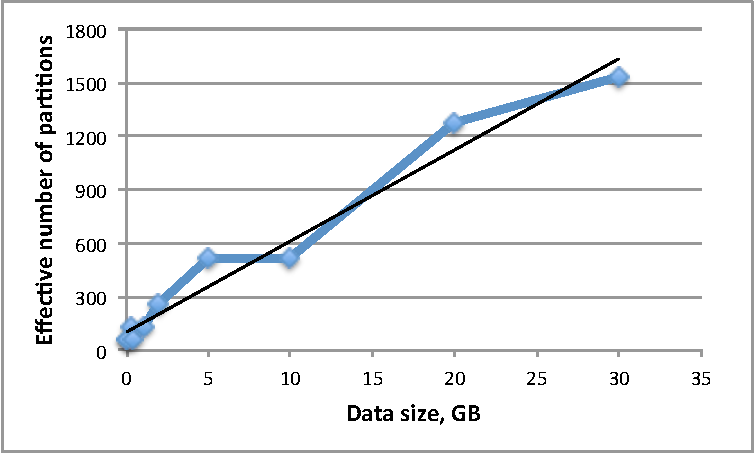
\includegraphics[width=2.7in]{figs/partsfit.pdf}
\vspace{-0.1in}
  \caption{Effective number of partitions.}
  \label{fig:partsfit}
\vspace{-0.1in}
\end{minipage}
\begin{minipage}{3in}
  \centering
  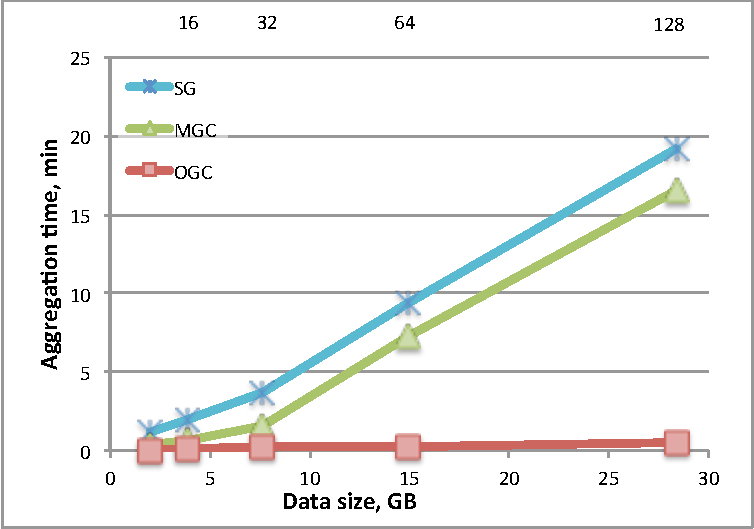
\includegraphics[width=2.7in]{figs/tgroupu_warm.pdf}
\vspace{-0.1in}
  \caption{\insql{TGroup} with \insql{All} (warm start).}
  \label{fig:tgroupu}
\vspace{-0.1in}
\end{minipage}
\end{figure*}

\begin{figure*}[t]
\centering
\begin{minipage}{3in}
  \centering
  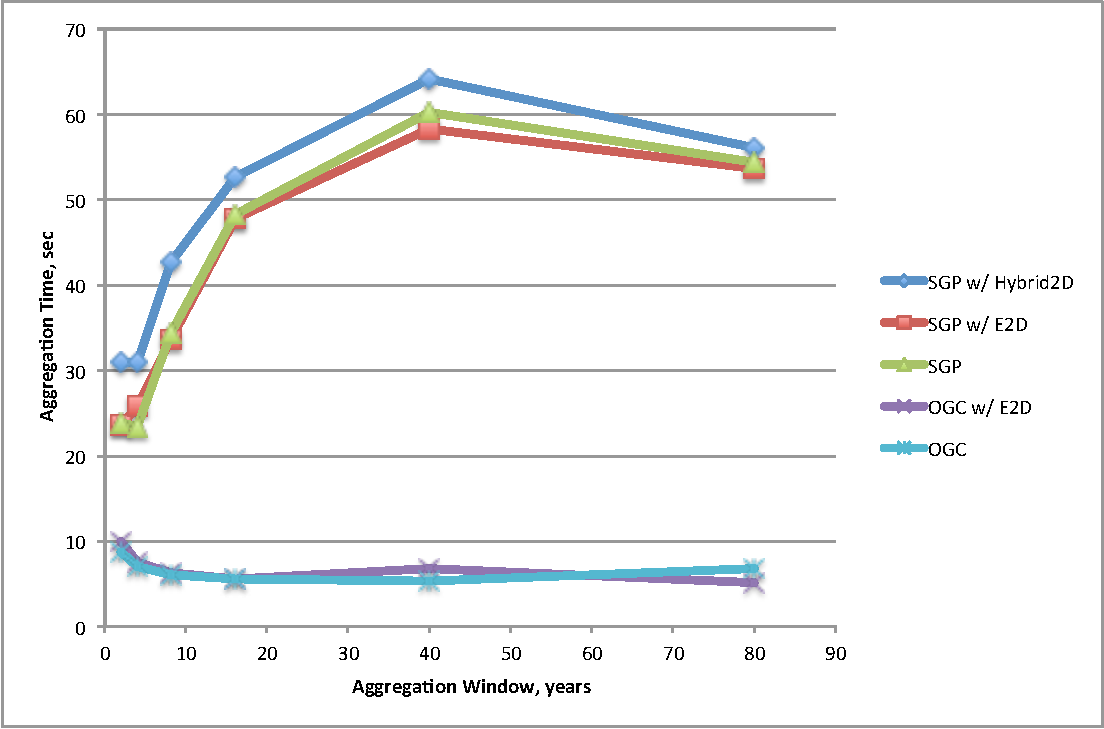
\includegraphics[width=2.7in]{figs/tgroupewidth.pdf}
\vspace{-0.1in}
  \caption{\insql{TGroup} by width, nGrams.}
  \label{fig:tgroup_width}
\vspace{-0.1in}
\end{minipage}
\begin{minipage}{3in}
  \centering
  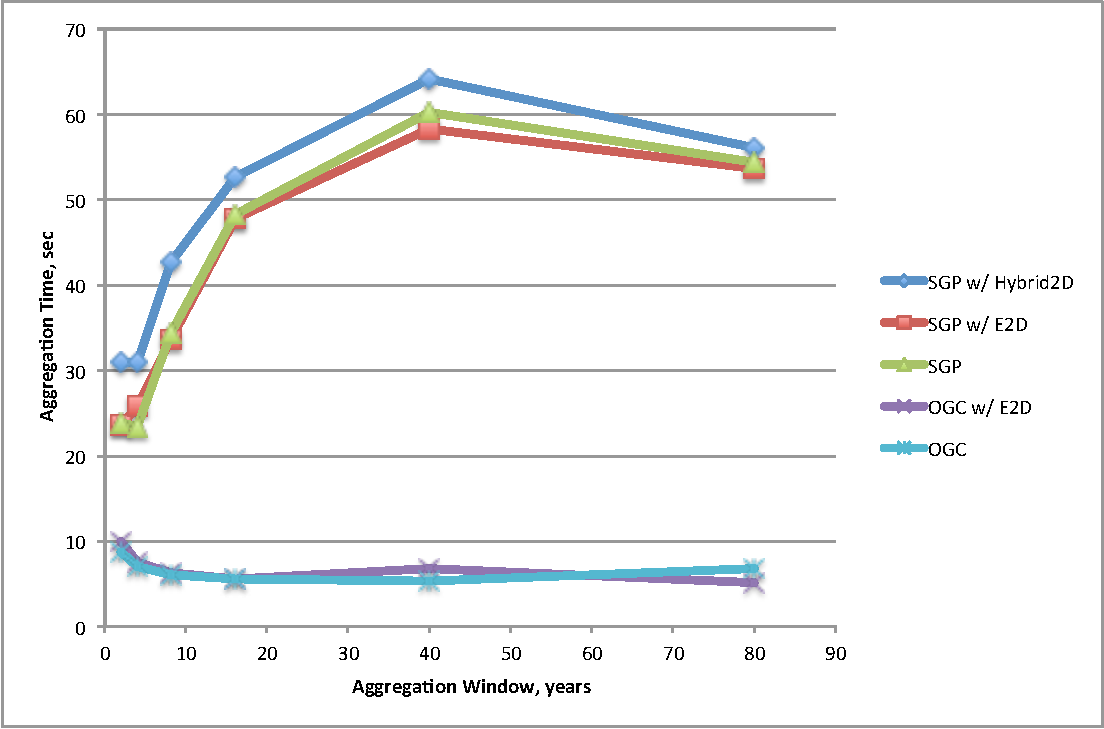
\includegraphics[width=2.7in]{figs/tgroupewidth_dblp.pdf}
\vspace{-0.1in}
  \caption{\insql{TGroup} by width, DBLP.}
  \label{fig:tgroup_width_dblp}
\vspace{-0.1in}
\end{minipage}
\end{figure*}

\begin{figure*}[t!]
\centering
\begin{minipage}{3in}
  \centering
  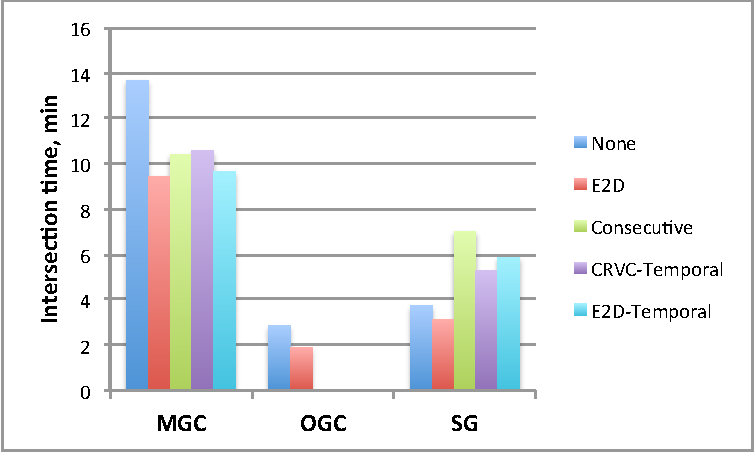
\includegraphics[width=2.7in]{figs/tand_parts.pdf}
\vspace{-0.1in}
  \caption{\insql{TAnd} by partition strategy, nGrams.}
  \label{fig:tand_parts}
\vspace{-0.1in}
\end{minipage}
\begin{minipage}{3in}
  \centering
  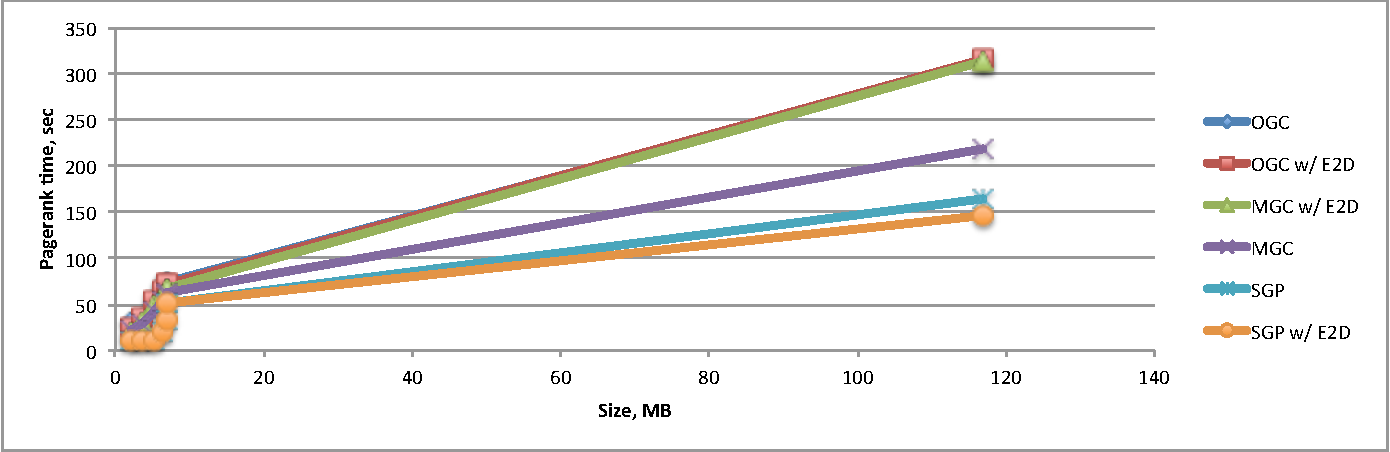
\includegraphics[width=2.7in]{figs/pagerank_dblp.pdf}
\vspace{-0.1in}
  \caption{PageRank time, DBLP.}
  \label{fig:pagerank_dblp}
\vspace{-0.1in}
\end{minipage}
\end{figure*}

Figure~\ref{fig:partsfit} complements Figure~\ref{fig:numparts}, in
which we presented the impact of number of partitions on the overall
performance.  In Figure~\ref{fig:partsfit} we show the linear trend
between the data size and the number of partitions that leads to
fastest execution.  The linear equation this fit produces is used in
the partition estimator during graph loading, except for very small
data sizes.

In Figure~\ref{fig:tgroupu} we show that \insql{TGroup} with
\insql{All} semantics exhibits the same behavior in all data
structures as \insql{TGroup} with \insql{Any} semantics in
Figure~\ref{fig:tgroupe}.  This is to be expected as both \insql{All}
and \insql{Any} use the same group by operation on the data, but with
different restrictions after grouping.

Another aspect of aggregation is the impact of an aggregation width.
Consider Figures~\ref{fig:tgroup_width} and
\ref{fig:tgroup_width_dblp} for the nGrams and the DBLP datasets,
respectively.  We fix the graph interval (128 and 80 snapshots,
respectively) and vary the width in powers of 2 up to total size.  For
each data structure we picked the most efficient partition strategy
based on the experiment in Section~\ref{sec:exp:tgroup},
Figure~\ref{fig:tgroupeparts}.  Observe that OGC and MGC are nearly
insensitive to the aggregation width, with small gains as the width
increases.  In contrast, SG performance logarithmically worsens as the
width increases in the DBLP dataset, but is largely unchanged for the
width values we evaluated in the nGrams dataset.

Figure~\ref{fig:tand_parts} complements Figure~\ref{fig:tandall}.  We
show that, similar to aggregation, partitioning improves performance
for temporal joins.  This finding is expected because co-partitioning
of two graphs along the same criteria improves the structural grouping
operation that is carried out. E2D partition strategy provides the
best performance, but the difference between it and the hybrid
strategies is not significant.

Finally, Figure~\ref{fig:pagerank_dblp} shows PageRank performance on
the DBLP dataset. Due to the very pronounced skew in the DBLP dataset,
the number of snapshots was drawn from the most recent to the left on
the timeline.  The same number of partitions was used for MGC/OGC
because the data size did not differ significantly between different
time intervals.  The general trend observed is the same as in the
nGrams dataset, with the only difference that at these small sizes the
E2D strategy does not produce an improvement in performance for MGC
and OGC.
